%!TEX encoding = UTF-8 Unicode
\documentclass{jsarticle}
\usepackage[dvipdfm]{graphicx}
\usepackage{url}

\begin{document}

%図番号に節番号を付加。節番号-図番号(図番号は節ごとに付ける)。
%http://www.biwako.shiga-u.ac.jp/sensei/kumazawa/tex/011.html
 \makeatletter
    \renewcommand{\thefigure}{
    \thesection.\arabic{figure}}
    \@addtoreset{figure}{section}
  \makeatother

%表番号に節番号を付加。節番号-図番号(表番号は節ごとに付ける)。
%http://www.biwako.shiga-u.ac.jp/sensei/kumazawa/tex/011.html
  \makeatletter
    \renewcommand{\thetable}{%
    \thesection.\arabic{table}}
   \@addtoreset{table}{section}
  \makeatother

\title{コンパイラ実験 レポート}
\author{03-130452 伏見遼平}
\maketitle


\section{達成度に関する報告}

字句解析器, 構文解析器, コード生成器すべてが完成した。すべてのテストデータ (basic\_tests, intapp\_tests) について正しい出力が得られた。

\section{追加課題}

何もしていない。

\section{実行速度}

gcc, gcc -O3, cogen の各コマンドで実行した速度の比較グラフを図3.1に示した。最適化をつけていない gcc よりも1.5 倍程度遅いことがわかる。

\begin{figure}[htbp]
\begin{center}
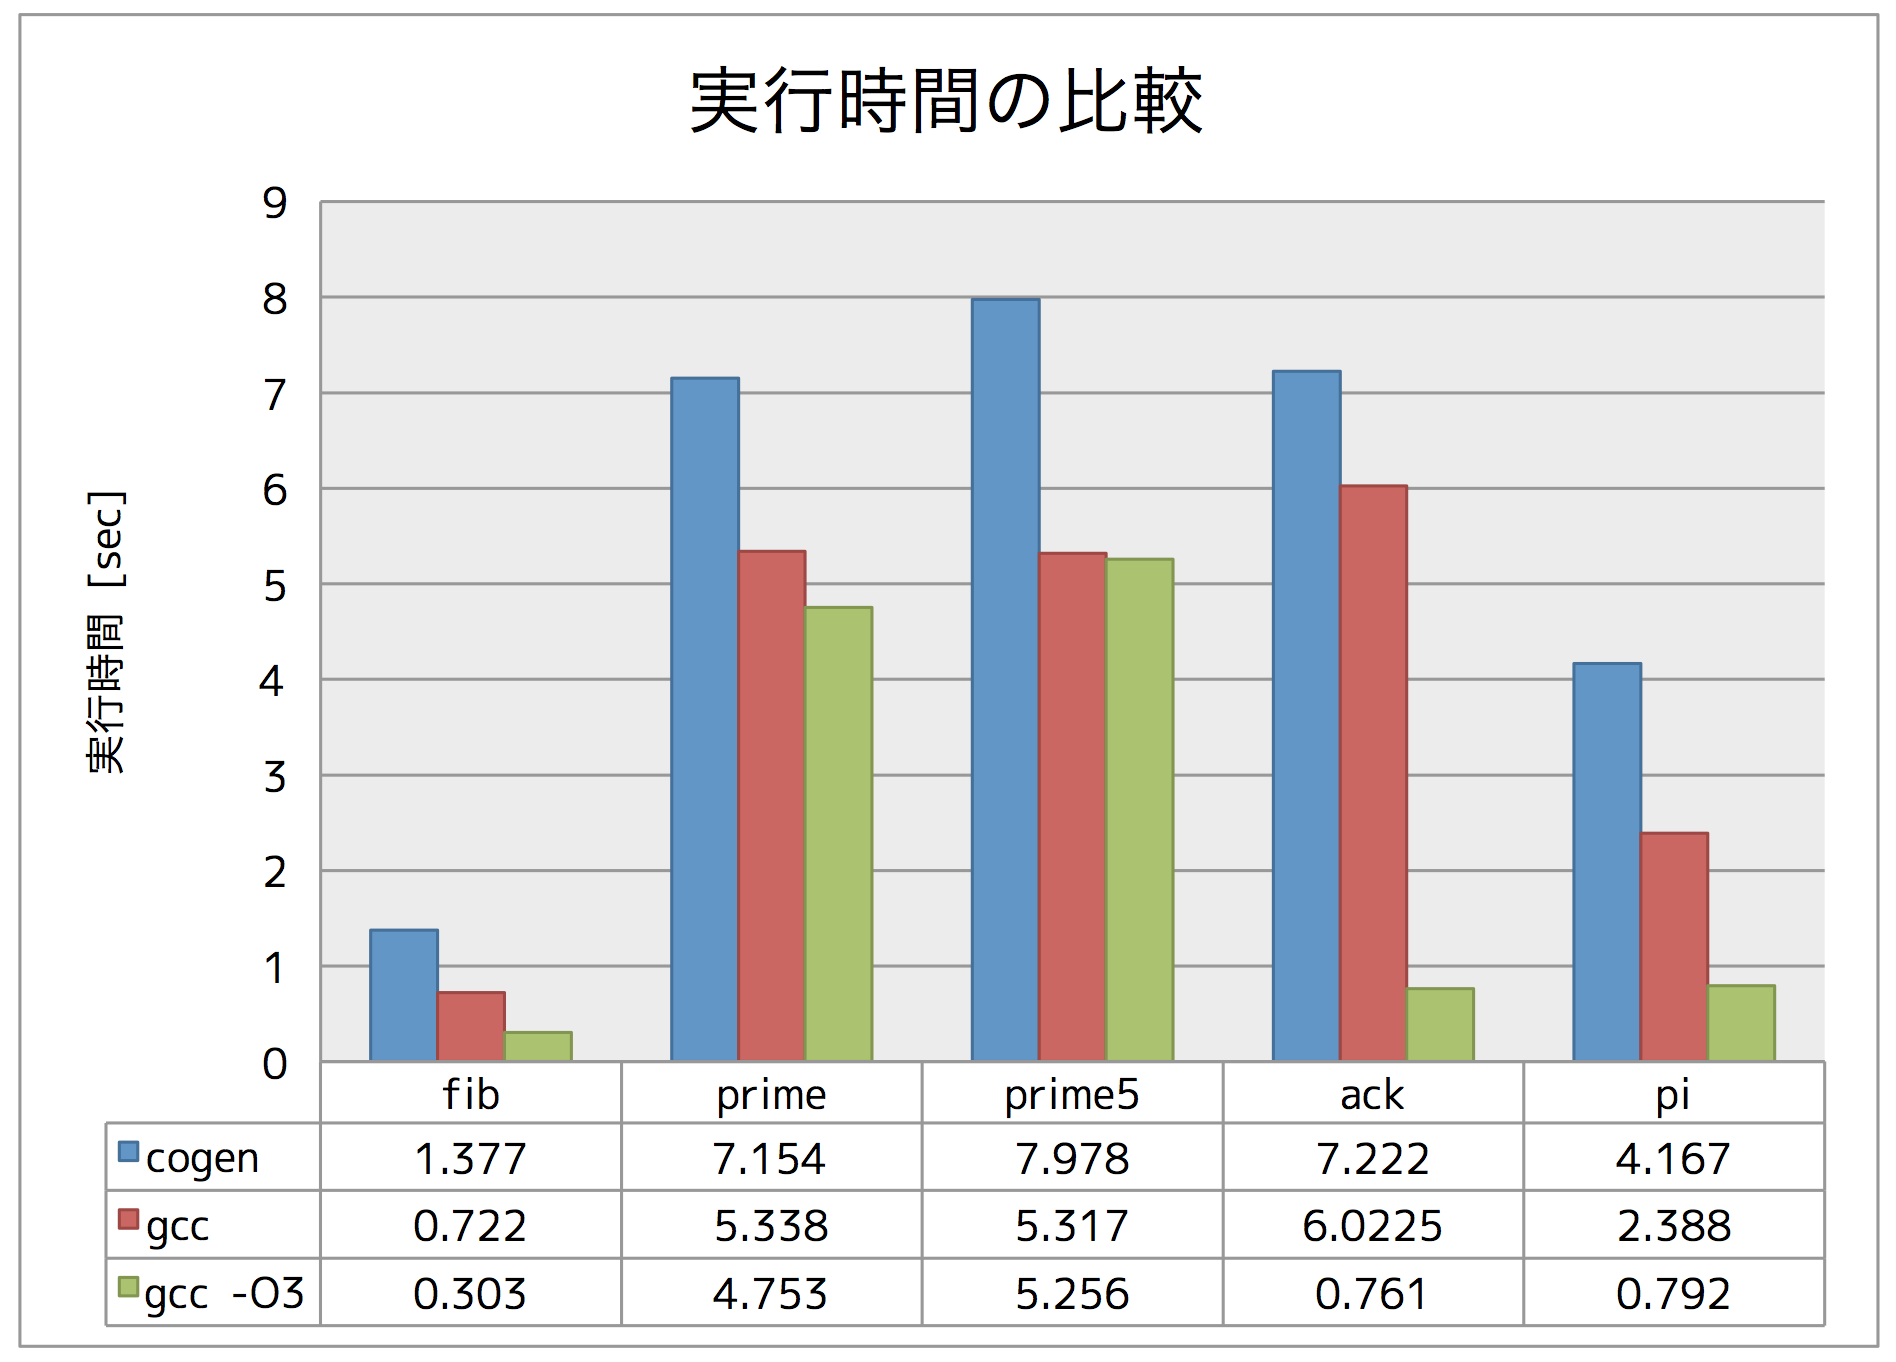
\includegraphics[width=12cm,clip]{result.png}
\end{center}
\caption{グラフ}
\label{fig:グラフ}
\end{figure}

\section{コード生成器の工夫}

コード生成器は、環境と連携しながらコードを生成するように設計した。具体的には、複合文 (compound\_stmt) ひとつひとつをスコープとして環境を割り当て、各複合文の中で定義されたローカル変数とメモリアドレスのタプルを環境がリストとして持てるようにした。この割り当てはコード生成器が動く前に行われる。コード生成器は、それぞれの変数や部分式が出てくるたび、そのメモリアドレスを環境に問い合わせればよいので、メモリアドレスの割り当てを気にせずに、コード生成を行えばよい。

\section{要望}

basic\_tests の中に、割る数が負であるような割り算のテストケースがなく、 basic\_tests が通過するのに、intapp\_tests が通過しない例があり、バグの追求に時間がかかった。もちろん、必要な部分には自分でテストを書くべきではあるが、basic\_tests の中に揃っているとスムースであった。

\end{document}